\part*{Introduction}
\addcontentsline{toc}{part}{Introduction}
\markboth{Introduction}{Introduction}

\vspace*{\fill}
\epigraph{\enquote{  Pamphlétaire !\ldots  Ah ! je suis autre chose, pourtant… mais si je suis pamphlétaire, moi, je le suis par indignation et par amour ; et mes cris, je les pousse, dans mon désespoir morne, sur mon Idéal saccagé !\ldots  }}{\textit{Léon Bloy, Le Bon Conseil, Belluaires et porchers Paris, 28 mai 1892. }}

\vfill\clearpage
\chapter{Préliminaires}
Cette étude se propose d'analyser le genre du pamphlet avec des méthodes stylistiques et textométriques. Un des objectifs de ce travail est de tirer parti des méthodes computationnelles pour vérifier à une plus grande échelle certaines hypothèses sur les spécificités du genre pamphlétaire issues d'analyses stylistiques. Le pamphlet comme sujet de recherche fut longtemps déconsidéré, étant situé en marge de la littérature dite classique. Le pamphlet, par sa violence extrême, ses sujets de controverses d'une actualité dépassée ou son parfum de scandale, n'était pas voué à conserver une valeur littéraire quelconque, ce qui peut expliquer un certain désintérêt pour son étude. Il y eu un regain d'intérêt pour ce champ d'étude avec le travail de Marc Angenot sur la typologie pamphlétaire \footcites{angenot_parole_1982} dont notre propos se voudra être un prolongement par le déploiement de méthodes computationnelles. Ce travail s'appuiera notamment sur les domaines de la qualification et de la classification des genres à l'aune des humanités numériques.

Au tournant du XIX\ieme siècle, une forme nouvelle de littérature est apparue. Elle a considérablement marqué la vie politique française, a révélé ou fantasmé des scandales d'état, a détruit des réputations, a engendré des monuments littéraires pour finalement péricliter dans la seconde moitié du XX\ieme siècle jusqu'à quasiment disparaître de nos jours. Cette littérature nouvelle fut le pamphlet. Phénomène littéraire, ambigu et protéiforme, le pamphlet connu son âge d'or de 1868 à 1968 et fut un marqueur fort de la fin du XIX\ieme 
 siècle agité de la vie littéraire et médiatique française.

L'analyse du discours moderne en littérature s'est considérablement développée sur l'étude des formes canoniques de la fiction et de la poétique; la littérature de combat dont le pamphlet fait partie, peut sembler être le parent pauvre de cette recherche. La nature même du pamphlet comme écrit de circonstance (dont la littérarité passe souvent au second plan d'une volonté persuasive) se démarque fortement des formes classiques de la littérature (des écrits pour durer dont la littérarité est au premier plan). Une difficulté supplémentaire s'ajoutant, pour étudier le phénomène pamphlétaire, est que ce champ d'étude n'est pas clairement circonscris et ce pour plusieurs raisons : le qualificatif de pamphlet est utilisé par une multitude d'acteurs différents et parfois récusé par les auteurs eux-mêmes. Aussi les distinctions de la forme du pamphlet, face à d'autres modèles plus anciens, tel que la \textit{diatribe}, \textit{l'opuscule}, la \textit{brochure}, le \textit{brûlot} et de nombreux autres encore, ne sont pas d'une évidence formelle. Nous proposons dans cette présente étude d'ouvrir des pistes de recherche de définition du genre pamphlétaire en utilisant des méthodes quantitatives en soutien à une analyse stylistique. Cette étude part du présupposé que le style propre d'écrivains se combine aux exigences du genre littéraire dans lequel il écrit, et que ces inclinaisons à écrire dans un genre donné et d'une certaine manière, peut correspondre à définir certains aspects spécifiques de ce genre.

\chapter{Historiographie du pamphlet}

Une longue tradition de texte polémique et satirique existe en France bien avant la Révolution française et l'apparition du pamphlet, on peut citer les \textit{mazarinades}, les \textit{pasquinades}, les \textit{libelles}, \textit{diatribes}, les \textit{placards}, \textit{brulôts} et bien d'autres dont le pamphlet se retrouve en être une forme héritière, nouvelle et concurrente.
Le pamphlet est un phénomène littéraire circonscris dans une période historique, le XIX\ieme siècle français. Avec les différentes lois régissant la liberté de la presse, et la massification des publications, ce siècle fut propice au développement d'une littérature polémique considérablement plus violente que sous l'ancien régime. Les conditions de développement historique du pamphlet furent étudiés par Cédric Passard dans \textit{L'Âge d'or du pamphlet}\footcites{passard_lage_2015}. De nombreux facteurs techniques, politiques et moraux permettent, non pas d'expliquer, mais de se renseigner sur le développement fulgurant des pratiques politiques et culturelles nouvelles de \textit{l'écrit de combat}.

L'usage du mot pamphlet est une nouveauté pour le XIX\ieme siècle français, de nombreuses autres formes synonymes avaient cours sous l'ancien régime. Sans forcément supplanter ces mots (le terme brochure resta concurrent mais bien plus général durant l'ensemble du XIX\ieme siècle) le terme pamphlet permis de définir un type spécifique divergeant des précédents synonymes évoqués et des modèles plus anciens de la satire et de la polémique. 

\begin{figure}[H]
\centering %
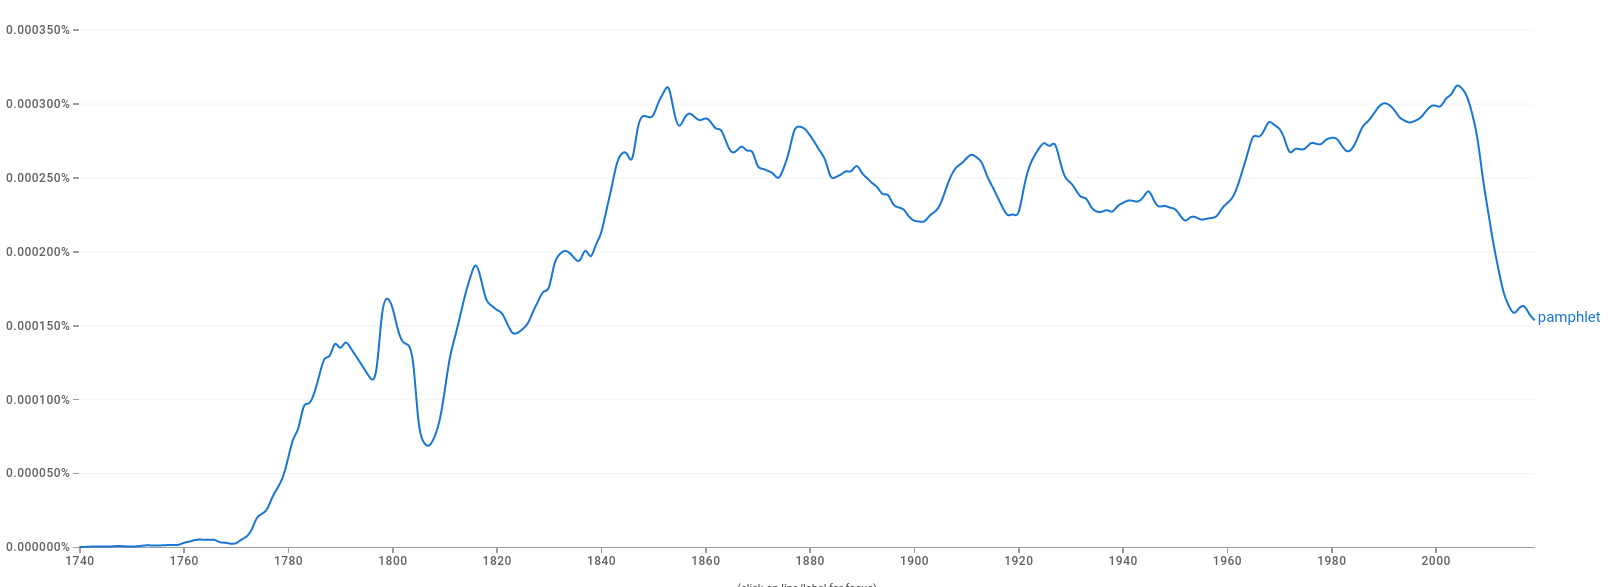
\includegraphics[width=1\textwidth]{img/google_ngramviewer_pamphlet_french_2019.png}
\caption{\textit{Visualisation de la fréquence d'emploi du terme pamphlet de 1740 à 2019, Google ngram Viewer, french corpus 2019}}
\label{fig:googlengram}
\end{figure}

La figure \textit{\ref{fig:googlengram}} montre l'ascension spectaculaire du terme \textit{pamphlet} de la fin du XVIII\ieme au début du XIX\ieme siècle. Il est intéressant de noter que certaines baisses de fréquence du mot ont l'air d'être directement corrélés aux périodes politiques propices à des lois encadrant strictement la presse. Sur la figure nous constatons trois pics baissiers qui peuvent correspondre aux période de la Terreur, de la Terreur blanche (sous la 1\iere Restauration avec la loi du 9 novembre 1815 sur les cris et écrits sédicieux \footcites{quensoi_de_la_hennerie_les_1925} qui fut adouci par la loi du 17 mai 1819) et de la seconde Restauration jusqu'aux ordonnances de juillet (dont la première ordonnance restreignait encore plus les libertés de la presse) et la révolution des Trois Glorieuses.

Sur la polysémie du mot pamphlet, le \textit{Dictionnaire de l'Académie française} donne à ce propos la définition suivante du terme pamphlet de la 4\ieme  édition de 1762 jusqu'à la 6\ieme  édition de 1835 : \enquote{\textit{Mot Anglois, qui s'emploie quelquefois dans notre langue, et qui signifie Brochure.}}\footcites{francaise_dictionnaire_nodate}. À l'entrée \textit{Brochure} de la 2\ieme  édition : \enquote{\textit{Petit ouvrage de peu de feüilles, qui n'est pas relié comme un Livre ; mais qui est seulement broché}}. Cette association du mot pamphlet à celui de brochure est présente jusqu'à la 8\ieme édition de 1935. Nous voyons que le rapport des deux termes est établi par la similitude de l'objet papier et non par son contenu bien qu'une grande partie des brochures ait pu traiter de politique. Paul-Louis Courrier relate dans \textit{le Pamphlet des pamphlets} son procès perdu à cause de l'ambiguïté du terme pamphlet entre écrit court et écrit injurieux, les contemporains du XIX\ieme siècle employaient le terme de pamphlet pour un grand nombre de texte divers et pour des raisons toutes aussi diverses et hétérogènes. 

\section{Une étymologie d'origine médiévale}

L'origine du terme à longtemps été controversée. Le \textit{Trésor de la Langue Française informatisé}\footcites{noauthor_tlfi_nodate} (TLFi) fait remonter la première occurrence du terme de pamphlet à Henri D'Andeli dans son poème la \textit{Bataille des VII Arts} de la moitié du XIII\ieme siècle, \textit{\enquote{La fu li sage Chatonez, Avionès et Panfilès}}.\footcites{henri_dandeli_oeuvres_1881} La forme \textit{Panfilès} est issue de Pamphile, suivant une évolution linguistique par nominalisation d'un nom propre par antonomase. Il existe plusieurs exemples de ce processus en Ancien Français, comme le recueil de fables attribué à Ésope se nomme \textit{\enquote{Isopet}} ou \textit{\enquote{Esopet}} comme l'\textit{\enquote{Avionès}} ou \textit{\enquote{Avionet}} est un poème d'Avianus et le \textit{\enquote{Chatonez}} ou \textit{\enquote{Catonet}} est un poème de Caton\footcites{morawski_pamphile_1917}. Ainsi le \textit{\enquote{Panfilès}} ou \textit{\enquote{pamphilet}} est le résultat d'une antonomase de Pamphile, désignant un ouvrage. \textit{le Pamphilus de amore}, \textit{Pamphile ou l'art d'être aimer} est une comédie latine très courte de 780 vers datant du X\ieme siècle, dont l'origine oscille entre la France et l'Espagne. Nous ne nous attarderons pas sur ce poème mais simplement, le sujet est d'une ironie assez marquée car le protagoniste éponyme, par le viol de Galatée, l'objet de son désir amoureux, échoue en amour. Cette comédie eu une grande influence dans toute l'Europe et on en retrouve une belle part dans l'inspiration du \textit{Roman de la Rose} et chez Geoffrey Chaucer, grand littérateur anglais du XIV\ieme siècle\footcites{morawski_pamphile_1917}. Le lien entre cette comédie et le genre du pamphlet se profile par deux prédicats communs, l'usage de l'ironie et la concision de l'ouvrage. La dimension européenne de la diffusion de cette comédie donne lieu, en 1344, au terme \textit{panfletus} du latin médiéval d'Angleterre qui se transforme en 1387-8 en \textit{pampflet} : \enquote{\textit{désignant parfois plus particulièrement une brochure sur un sujet d'actualité, éventuellement de politique ou propre à la controverse}} toujours d'après le TLFi. Les brochures, comme les opuscules sont de petits livrets qui circulaient par des canaux de diffusion non contrôlés par les instances politiques. La rapidité d'impression d'un ouvrage est associable à sa circulation clandestine, d'où la part importante de pamphilet à dimension ironique, satirique ou polémique. Cela préfigure notre acception moderne du pamphlet comme un texte utilisant les registres de l'ironie et de la polémique et de peu de pages.

\section{Libelle et pamphlet à l'époque moderne}
Le mot apparaît en français pour la première fois en 1653 dans \textit{Les voyages et observations du sieur de La Boullaye Le Gouz}\footcites{la_boullaye-le_gouz_les_1653} au sujet de l'abolition du vieux parlement anglais par le roi Charles X qui le \enquote{\textit{déclara pamphlet}}\footcites{la_boullaye-le_gouz_les_1653}. L'auteur précise en marge le sens du mot comme : \enquote{\textit{Pamphlet en Anglais est un papier barbouillé qui n'est bon à rien et revient en notre langue au mot de festu}}\footcites{la_boullaye-le_gouz_les_1653}. Un \textit{fétu} désignant alors au sens figuré dans le TLFi \enquote{\textit{Une chose sans importance, d'une valeur minimale}}. Voilà une nouvelle dimension du terme pamphlet qui met en évidence la connotation dépréciative qu'il porte en son sein dès son emploi dans la langue anglaise et au moment de son apparition dans un texte en français. Durant tout le XVI\ieme siècle, le terme pamphlet reste encore propre à la langue anglaise et ses rares occurrences en français sont toujours le fruit d'un emprunt direct à l'anglais. Nous retrouvons aussi dans les \textit{Mémoires et observations faites par un voyageur en Angleterre}\footcites{misson_de_valbourg_memoires_1698} de 1698 où à l'entrée \textit{libelle} une définition colloquée à celle de pamphlet écrit dans la marge pour : \enquote{\textit{papiers imprimez, où chacun prend la liberté de dire beaucoup de choses sur les Affaires de l'État \& de publier toutes sortes de nouvelles. Je ne dis pas que chacun s'émancipe impunément à dire tout ce qu'il pense, mais je dis qu'on y prend une très grande liberté. [. . .] L'extrême douceur du Gouvernement donne lieu à ces sortes de Licences}}.\footcites{misson_de_valbourg_memoires_1698} Le terme voit son sens s'infléchir vers la connotation de diffamation et l'aspect sulfureux ou immoral de son propos.

\section{Un phénomène européen}
La genèse du \enquote{genre} pamphlétaire que nous connaissons au début du XX\ieme siècle tire bien sa source de ces libelles qui désignent conformément à son étymologie \textit{libellus} un petit livre ; l'exemple de cette définition de 1698 rejoint un état de fait qui concerne toute l'Europe depuis plus d'un siècle où l'imprimerie sert à la diffusion très large de courts feuillets en contournant les rapports traditionnels entre l'imprimé et les autorités. Ces feuillets sont des vecteurs de polémiques et de controverses exceptionnelles. Durant les guerres de Religion par exemple, une multitude variée de feuillets ont vu le jour tel les \textit{occasionnels}, les \textit{canards}, les \textit{mazarinades} et plus communément les \textit{placards}, Jean Guillemain parle lui, pour la fin du XV\ieme siècle, de la naissance \enquote{\textit{de l'écrit politique de masse}}\footcites{guillemain_livre_nodate}. Cette révolution de l'écrit subversif passe évidemment par le taux extrême d'impression et de réplication que permet alors l'imprimerie ; on compte plus de 3700 éditions différentes des ouvrages de Martin Luther de son vivant\footcites{guillemain_livre_nodate}. Plus au sud, à Venise en 1606, après l'interdit prononcé par le pape Paul V contre la République de Venise, une guerre de l'information fut menée dans des proportions hors-normes pour l'époque. Filippo de Vivo a écrit à ce sujet : \enquote{\textit{Ces écrits ont animé un moment polémique et éditorial sans précédent en Italie, comparable à des conflits comme la Fronde française ou la guerre civile anglaise. Jamais un si grand nombre de textes n'avaient paru en si peu de temps pour mettre en question les rapports entre Église et État, les limites de l'autorité ecclésiastique, la légitimité et l'origine du pouvoir séculier}}\footcites{vivo_chapitre_2016}. 
L'ensemble de ces textes se publiaient sous anonymat ou pseudonymat. Mais ces formes antérieurs sont bien une étape nécessaire vers l'avènement du \enquote{genre} pamphlétaire par sa distinction de la satire, les cibles des ces textes sont rarement contre des modèles, à la manière des \textit{Caractères} de Théophraste, où sont dépeint par exemple le type de l'avare ou de l'orgueilleux, mais bien contre des personnes et des institutions. Le pamphlet dans son évolution concomitante des libelles perdit sa dimension satirique (au sens de la satire dite sociale) en conservant principalement celles polémique et ironique.

\section{Apparition en français de pamphlet}
Une des premières apparitions du terme de pamphlet en tant qu'acception française dans un texte se trouve en 1762, dans le premier tome des \textit{Mémoires secrets de Bachaumont}\footcites{bachaumont_memoires_1783} le terme de pamphlet y apparaît quatre fois, le plus souvent accolé au terme de libelle qui lui compte onze occurrences. Nous présentons ici deux extraits de ces premières apparitions en français du mot pamphlet.\\\par
\textit{Il étoit déja connu par la Vision de Sr. Paliffot, pamphlet très-satirique (Des femmes de la plus haute considération y étoient tournées en ridicule) qui lui avoit fait faire quelque séjour à la Bastille} p.48\footcites{bachaumont_memoires_1783}\\\par

\textit{8 Décembre 1762. Arrêt rendu par le conseil souverain du Parnasse. Cet écrit est une plaisanterie contre l'insolent libelle de M. Poinsiner : elle est de M... Il ne méritoit pas qu'un plus digne athlete descendît dans la lice. C'est un pamphlet médiocre, comme l'ennemi qu'on combat} p.154\footcites{bachaumont_memoires_1783}\\

C'est ainsi à partir de la seconde moitié du XVIII\ieme siècle que le pamphlet progressivement s'ajoute au terme de libelle dont la signification, depuis le XV\ieme siècle, évolua d'un acte à valeur juridique à un \enquote{\textit{écrit généralement court, diffamatoire, dirigé contre une personne, un groupe de personnes, une corporation}} d'après le TLFi. Au XIX\ieme, la différenciation du pamphlet face au libelle s'affermit car même s'ils sont souvent synonymes, c'est bien deux phénomènes distincts. Seulement l'étendu du terme pamphlet va lentement supplanter celui de libelle dans l'usage de la langue. Mais cette évolution du vocabulaire ne change pas la connotation diffamatoire, ordurière ou scandaleuse de cette littérature d'actualité. C'est encore au XIX\ieme siècle que le pamphlet évolua avec la lente apparition de la figure du pamphlétaire comme écrivain écrivant publiquement sans anonymat. Les différentes lois de censure de la presse n'empêchèrent pas le pamphlet d'avoir un véritable essor et malgré une très forte accusation de médisance publique, sa littérarité fut de plus en plus reconnu comme avec \textit{Napoléon le petit} de Victor Hugo par exemple. De fait le pamphlet devient l'oeuvre d'écrivains reconnus.

\section{Son développement au XIX\ieme siècle}
La polysémie du mot est d'ailleurs rapportée dans \textit{le Pamphlet des pamphlets} de Louis-Paul Courrier\footcites{courier_pamphlet_1824}. Durant le siècle des révolutions, le mot va lentement supplanter d'autres synonymes de texte polémique et violent. Son emploi au sens moderne est associé à la clandestinité de sa diffusion qui est souvent illicite, pour la première moitié du XIX\ieme siècle, les auteurs des pamphlets restent anonymes ou sous pseudonymat pour se prémunir de poursuites judiciaires. Sa grande popularité comme format court traitant d'actualité est facilitée par les évolutions techniques et économiques de l'imprimerie. Son développement est concomitant avec le développement de la presse française\footcites{feyel_presse_2007}. En mai 1868, Henri de Rochefort, ancien chroniqueur au \textit{Figaro}, lança son hebdomadaire \textit{La Lanterne}, brochure de 62 pages en petit format in16 dont le succès fut immédiat avec un tirage à 120 000 exemplaire dès le premier numéro. L'année suivante le 4 mai, Henri de Rochefort participa aussi à la fondation du quotidien \textit{Le Rappel}\footcites{barbieux_rappel_1869} de la famille de Victor Hugo, dont Victor Hugo y est indirectement associé. En 1880, le quotidien tirait 50 000 exemplaires. Néanmoins des freins à l'hégémonie de ce genre existent ; les variations des lois sur la liberté de la presse force nombre de pamphlétaires soit à cesser l'impression de leur brochure soit à s'exiler comme Henri de Rochefort qui parti pour la Belgique. La loi libérale du 11 mai 1868 sur la presse démantèle le précédent système transférant les pouvoirs de contrôle de la presse par l'administration à la justice. Cela eu comme conséquence de multiplier les procès à l'encontre des pamphlétaires mais sans réussir pleinement à diminuer le développement de la presse d'opposition. Une condamnation de ce genre est évoquée par Louis-Paul Courrier dans \textit{le Pamphlet des Pamphlets}. En 1870, 18 quotidiens politique parisiens fondée en 1868 diffusent au total 227 300 exemplaires\footcites{feyel_presse_2007}. La même année \textit{La Lanterne} est interdite, le quotidien \textit{La Marseillaise}\footcites{noauthor_marseillaise_1877} d'Henri Rochefort prend le relais. Cela montre bien que l'offre pamphlétaire répondait à une demande forte pour les lecteurs. Pour comprendre le succès éclatant de ce type de brochure, il faut savoir que \textit{La Marseillaise} et \textit{Le Rappel} sont (hors de trois quotidiens subventionnés par le gouvernement) les journaux les plus tirés. Avec la place hégémonique de cette nouvelle forme de brochure polémique et satirique, certains scandales politiques vont avoir une caisse de résonances énorme. Les exemples de l'affaire des souscriptions Baudin en 1869 sucscitée par la presse d'opposition et l'affaire de l'assassinat de Victor Noir, journaliste à \textit{La Marseillaise} par le prince Pierre Bonaparte, cousin de Napoléon III, lors d'un duel, ont montré l'impact qu'ont eu les pamphlets pour la société impériale. Henri de Rochefort écrivait au sujet de l'assassinat de Victor Noir dans \textit{La Marseillaise} : \enquote{\textit{J'ai eu la faiblesse de croire qu'un Bonaparte pouvait être autre chose qu'un assassin. J'ai osé m'imaginer qu'un duel loyal était possible dans cette famille où le meurtre et le guet-apens sont de tradition et d'usage}}. Ces lignes ont eu un retentissement extraordinaire et montrent la liberté de ton que s'accorde les écrivains pamphlétaires et la résonnance de leur textes dans la société française.

\section{L'Âge d'or du pamphlet}

D'autres scandales encore éclateront et furent amplifiés sous la plume de pamphlétaire comme le scandale de la corruption du canal de Panama en 1892 avec des pamphlets d'Édouard Drumont détaillant les ressorts du scandale dans son quotidien \textit{La Libre Parole}\footcites{drumont_libre_1892}. Enfin le développement de l'Affaire Dreyfus fut en grande partie porté par des pamphlétaires et certains pamphlets ont eu un retentissement pharamineux comme le très célèbre \textit{J'accuse} d'Émile Zola aujourd'hui étudié dans toutes les écoles. Pour définir cette période, un terme, \textit{le pamphlétarisme} fait son entrée dans \textit{le Grand Dictionnaire Larousse de 1877} : \enquote{\textit{pamphlétarisme — désigne la manie du pamphlet, l'emploi systématique du pamphlet pour attaquer, pour dénigrer}}\footcites{larousse_grand_1866}. Cédric Passard à traiter cette période de l'hégémonie du genre dans \textit{l'Âge d'or du pamphlet}\footcites{passard_lage_2015}.
Ainsi le pamphlet est partout, et est lu par tout le monde, c'est véritablement le triomphe du genre. Néanmoins l'image du pamphlet reste sulfureuse. Même si l'écriture de pamphlets s'est professionnalisé au même titre que le reste du journalisme, c'est surtout la période des professionnels du scandale. Le pamphlet entièrement sortie de la clandestinité atteint des sommets de lecteurs. En cela, il participe pleinement de cette fabrique moderne d'un nouveau lectorat qui englobe toutes les couches de la société : \enquote{l'opinion publique}\footcites{farge_dire_1992}. Ce sera avec les écrivains du début XX\ieme siècle comme Léon Bloy, Georges Bernanos ou Charles Péguy, que le genre sortira petit-à-petit de son aspect scandaleux de littérature souterraine et gagnera littérairement ses lettres de noblesse. Durant cette période, de nombreux journaux continueront d'utiliser le pamphlet comme arme idéologique tel \textit{l'Action française} ou d'autre mouvement comme celui des surréalistes et bien d'autres encore\footcites{passard_pamphlet_2009}.

\section{Déliquescence du genre}

Après la guerre d'Algérie et les révoltes de mai 1968, le genre du pamphlet à lentement disparu. Marc Angenot considère la fin de l'âge d'or du phénomène pamphlétaire en 1968 justement. La raréfaction du pamphlet depuis cette période et sa discrète déréliction peut s'expliquer par des phénomènes politiques et économiques, notamment les conséquences des Trentes glorieuses sur l'apaisement de l'opinion publique. Le pamphlet par son outrance verbale est moins populaire et plus facilement jugé sociétalement problématique. Quelques exceptions de survivance du genre apparaissent dans des portraits de personnalités politiques mais cela reste un phénomène circonscrit. D'autres tentatives d'actualisation du genre passent par la dissimulation du pamphlet dans une forme d'essai plus cognitifs comme l'exemple donné par Marc Angenot de \textit{La Trahison des Clers} de Julien Benda\footcites{angenot_parole_1982}.  La disparition des lois qui attentaient à la liberté de la presse et la mise en place de loi condamnant la diffamation ont probablement réussi à réduire considérablement les possibilités de diffusion de violence véhiculée sous la forme de pamphlet. Cédric Passard a étudié cette question de la disparition contemporaine du genre dans \textit{Le pamphlet meurt-il de liberté?}\footcites{passard_pamphlet_2009} et \textit{Les mutations du pamphlet dans la France contemporaine}\footcites{hastings_les_2009}. L'opinion partagée des chercheurs que nous avons convoqués pour résumer l'histoire passé du pamphlet est que son avenir passe par une mutation du genre tel qu'il ne recouvrira plus les spécificités qu'il lui était propre au début du XX\ieme siècle. Pour cette étude présente, nous ne chercherons pas à interroger l'homogénéité du genre pamphlétaire du point de vue diachronique dans le champ d'une linguistique historique du genre. En effet, nous voyons que le phénomène pamphlétaire est un phénomène littéraire qui a constament évolué et bourgeonné sous plusieurs formes, une étude de cette évolution historique ne recouvre pas notre sujet, nous nous intéréssons à la période la plus classique de son développement : la fin du XIX\ieme jusqu'au début du XX\ieme siècle. 
Après avoir retracer dans les grandes lignes l'histoire du pamphlet nous souhaitons établir ce qu'est le genre en littérature et en quoi le pamphlet peut-il s'y accoler.

\chapter{État de l'art}

\section{Qu'est-ce-que le genre ?, vers une définition du pamphlet ?}
Lorsque dans cette présente étude, nous écrivons \enquote{genre} pamphlétaire, nous insistons graphiquement sur les guillemets entourant le terme de genre du fait même que cette notion nécessite d'être clairement définie pour comprendre ce qui implique de parler d'un \enquote{genre} pamphlétaire et même si cela est possible.\par
La question de définition du genre en stylistique et plus largement en linguistique à de nombreux écueils. Bien qu'intuitivement la notion de genre en littérature classique est une catégorie bien établie, les linguistiques lui opposent de nombreuses subtilités. Dans les études linguistiques françaises le domaine de la linguistique de genre n'est pas un champ clairement délimité, il existe plusieurs écoles qui approchent cette question par des paradigmes distincts tel que les genres de discours, genres discursifs, genre de textes, genre textuels, genre de la parole ou encore types de textes ou styles de texte. Christophe Gérard dans son étude de \textit{Linguistique des genres}\footcites{gerard_linguistique_2019} propose de retracer les divers travaux de la linguistique textuelle dont la linguistique de genre est issue, il en ressort pour notre réflexion des notions directrices et empirique pour définir le genre. Le genre est une norme discursive distincte des normes idiomatiques, François Rastier lui, écrit que \enquote{les genres sont définis par l'interaction normée de composantes textuelles}\footcites{rastier_malrieu_nodate} En cela il appartient à une tradition discursive, chaque genre est avant tout un phénomène historique circonstanciable. Cette approche empirique permet de considérer le genre dans un aspect synchronique. L'appartenance d'un texte à une tradition discrusive tel qu'un genre ne s'oppose pas à l'appartenence d'autres traditions comme dans le cas d'hybridation générique où plusieurs traditions se mêlent au sein d'un même texte. Par exemple \textit{La France juive}\footcites{drumont_france_1888} d'Édouard Drumont se situe également (non au sens d'une stricte égalité mais de distributivité) entre l'essai cognitif et le pamphlet. Aussi cette recherche d'historicité des genres permets d'éviter l'écueil de nommer comme catégories génériques des catégories descriptives qui ne le seraient pas. L'exemple d'une catégorie descriptive n'indique rien de la tradition et de la séquence qu'elle comporte. En effet la description romanesque, la description satirique ou description poétique ne renvoient pas à un rapport générique, chacune de ces catégories issues de la description n'indiquent pas que la description soit un genre. La description ne défini pas un texte. La dénomination de genre doit être donc lié à l'historicité du genre. Christophe Gérard toujours, nous donne des exemples de genre dans cette acception précise : \enquote{\textit{la tragédie élisabéthaine, la tragédie classique, le sonnet baroque, le roman antique}}. Ainsi la tragédie en soi, le roman en soi sans borne diachronique n'est pas une réalité empirique mais une construction ou une reconstruction théorique. Le sonnet, la tragédie ou le roman en soi appartiennent alors à un champ générique (des familles de genre) fruit d'une théorisation réunissant des genres issues de traditions historiques. Un exemple de reconstruction apparait dans l'avant-propos de \textit{Les Polémistes français depuis 1789} de Pierre Dominique : \enquote{\textit{Dès que les hommes surent écrire, naquit le pamphlet qui, sans doute, commença par le graffiti injurieux et ordurier, et qui pouvait être illustré, la polémique orale suivant un chemin parallèle, d'où les pamphlets parlés, tels les Philippiques.}}\footcites{dominique_les_1962}. Nous comprenons l'acception du genre par cette visée de renommage de genre littéraire a posteriori mais comme nous développerons après, le genre du pamphlet en tant qu'objet linguistique dans notre étude ne sera compris que comme une réalité empirique et non comme un champ générique diachronique. 
Christophe Gérard reprend les travaux de Kuon et de Rastier pour affirmer qu'il y a pour les genres trois dimensions définitoires en tant qu'\enquote{\textit{objet idéal}} : la conception, la fonction et l'évolution \footcites{gerard_linguistique_2019}. La conception s'intéresse aux modalités du langage, à la rhétorique du texte, aux motifs, aux unités de sens. La dimension fonctionnelle renvoie aux actes de langage de la linguistique pragmatique tel que défini par Austin dans \textit{Quand dire, c'est faire}\footcites{austin_quand_1970} et déployé par Schaeffer \footcites{schaeffer_quest-ce_1989}. La dimension de l'évolution s'attache quant à elle à l'aspect diachronique du genre, c'est le propos de la linguistique historique des genres. Par exemple, l'ouvrage de M. Jalbert, \textit{De quoi l'essai est-il le nom ?}\footcites{jalbert_quoi_2013} s'attache à définir l'essai dans une perspective diachronique qui montre l'évolution dans le temps de ce genre. La dimension de la conception du genre d'un texte contient aussi les registres tel que défini par Douglas Biber et Susan Conrad \footcites{biber_register_2009} qui permet l'analyse des variétés lexicales et des relations syntaxiques.
Nous pouvons ajouter à cette définition tripartite du genre, une dimension verticale de classement, certains genres sont à rapprocher dans une famille de genres, le champ générique. François Rastier, dans \textit{Sémantique pour l'analyse}\footcites{rastier_malrieu_nodate}, écrit \enquote{Il faut reconnaître d'une part qu'il n'existe pas de texte sans genre, et en outre que tout genre relève d'un discours}\footcites{rastier_malrieu_nodate}. Cette hiérarchie entre champ générique, genre et discours se retrouve bien présenté dans \textit{Genres et variations morphosyntaxiques}\footcites{rastier_malrieu_nodate}. La \textit{figure \ref{fig:rastier_marlrieu_niveau_classification}} montre un exemple de ce classement verticale des textes et la place du genre au sein de celui-ci.
\begin{figure}[H]
\centering %
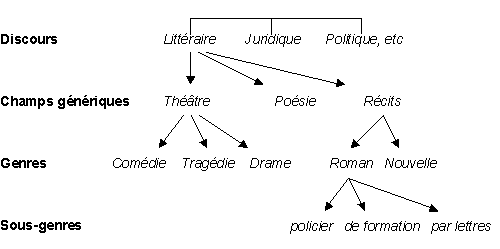
\includegraphics[width=0.8\textwidth]{img/MR_Genres1_niveau-declassification.png}
\caption{\textit{Niveau de classification défini par Rastier et Malrieu\footcites{rastier_malrieu_nodate}}}
\label{fig:rastier_marlrieu_niveau_classification}
\end{figure}


Marc Angenot, quant a lui propose une filiation générique du pamphlet sur des catégories essentiellement discursives. C'est ce que l'on peut observer avec la \textit{figure \ref{fig:angenot_niveau_inclusion_générique}}. Ces deux méthodes de classification du genre en ensemble et sous-ensemble montrent la richesse méthodologique et théorique de définition du genre littéraire.
\begin{figure}[H]
\centering %
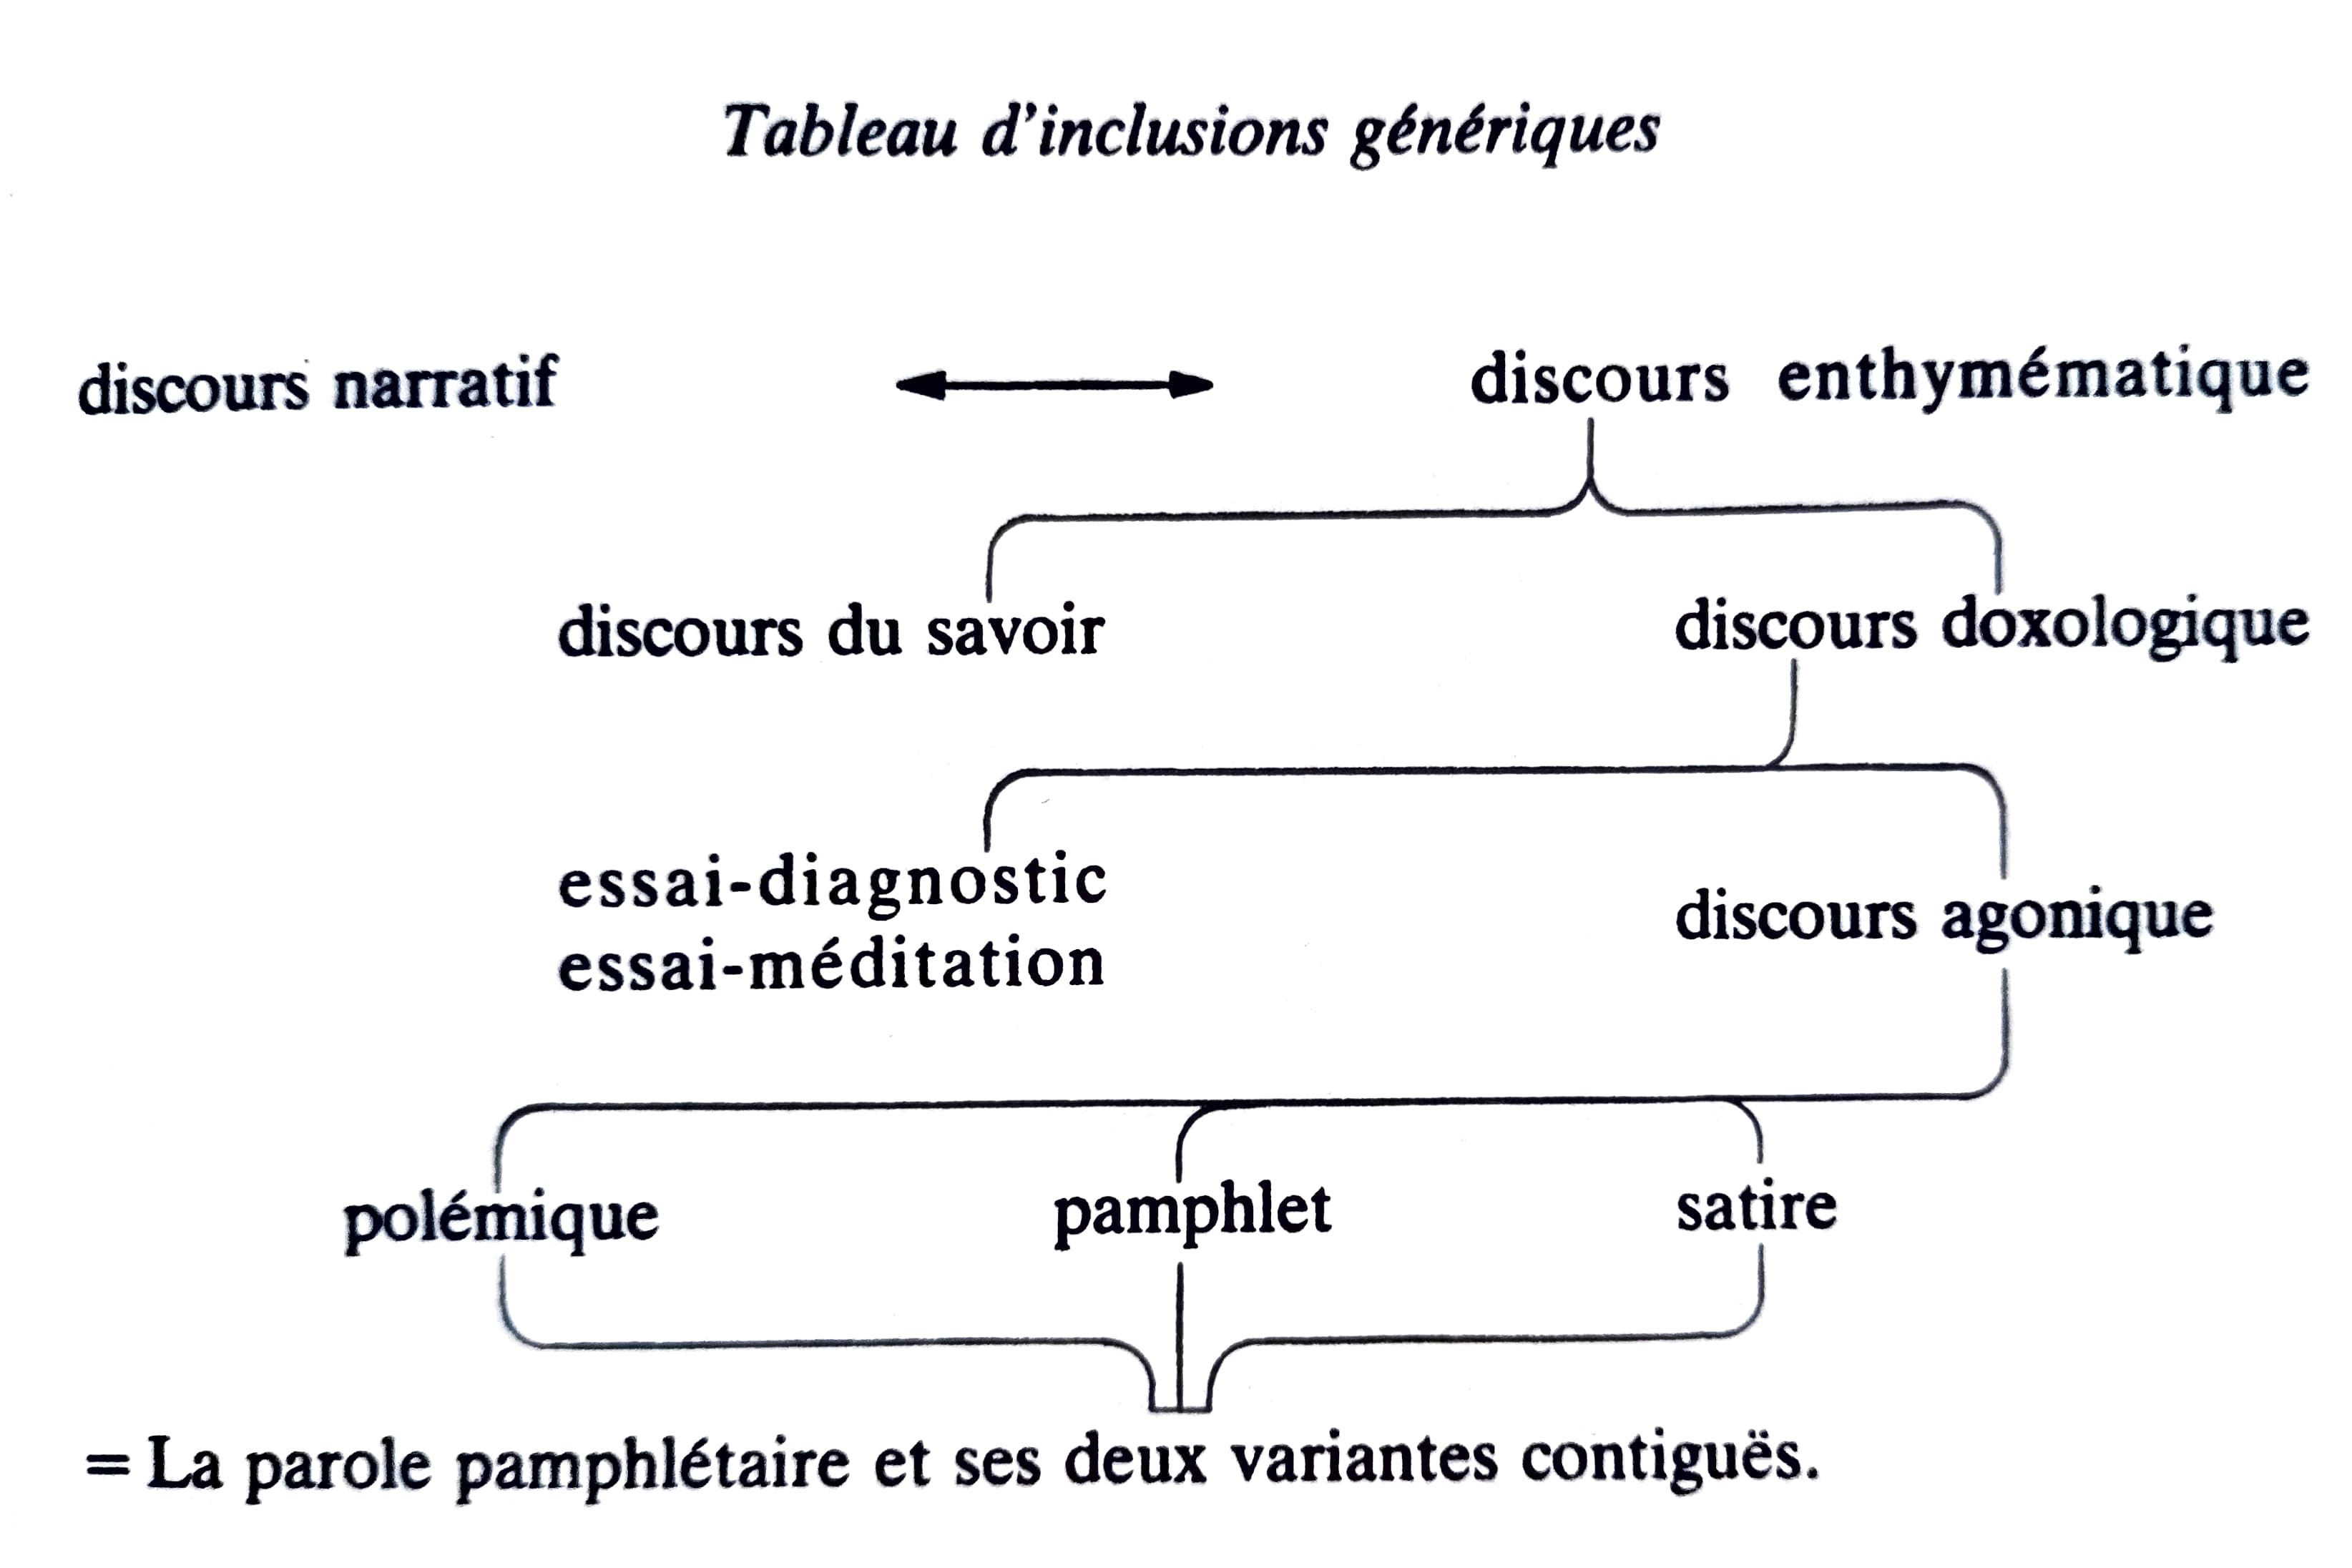
\includegraphics[width=0.65\textwidth]{img/fig_M_Angenot_tableau_inclusion_generique.png}
\caption{\textit{Niveau d'inclusion générique du pamphlet par Marc Angenot\footcites{angenot_parole_1982}}}
\label{fig:angenot_niveau_inclusion_générique}
\end{figure}
Ainsi nous observons le phénomène de genre comme catégorie s'insérant dans une hiérarchie d'ensemble. Une autre manière de définir le pamphlet peut passer par la définition d'un style collectif. Collectif à comprendre comme ensemble socioculturel, les pamphlétaires bien que ne se connaissant pas personnellement partagent un même air du temps. Marc Angenot d'ailleurs a dressé une typologie de la figure du pamphlétaire.
\section{Qu'est-ce-que le style ?}

La définition de la notion de style diffère en fonction du champ disciplinaire où l'on se place. Dans notre étude pluridisciplinaire nous empruntons la notion de style à la fois à la linguistique mais aussi à la stylométrie dont le mot même exprime l'étude de la mesure du style.
Notre recherche de traits formels spécifiques au \enquote{genre} pamphlétaire peux s'apparenter à une recherche d'un style collectif des textes étiquetés pamphlet. Rechercher des marques d'un style collectif suppose d'évincer les marques du style individuelle ou idiolecte. Si le style peut être compris comme \textit{la déviation d'une norme}, nous chercherons la norme de ces déviations dans les textes pamphlétaires. Notre approche de la notion de style est pluridisciplinaire et se situe au carrefour de la stylistique et de la stylométrie, une forme de linguistique de corpus appliqué avec de méthodes quantitatives. Dans la linguistique de corpus, le style est souvent défini comme la manière particulière dont un auteur ou un groupe d'auteurs utilise la langue pour communiquer, y compris les choix lexicaux, syntaxiques et sémantiques qui caractérisent leur production textuelle. Il peut être étudié à travers l'analyse de fréquences, de motifs récurrents, et d'autres caractéristiques linguistiques au sein de grands ensembles de textes. En stylométrie, le style se réfère aux propriétés linguistiques et statistiques distinctives qui permettent d'attribuer un texte à un auteur spécifique. Cette visée attributive nous intéresse particulièrement dans l'objectif d'une attribution non autoriale mais générique. En stylistique, le style se définit comme l'ensemble des choix linguistiques et stylistiques qu'un écrivain ou un locuteur fait pour s'exprimer de manière particulière. Cela inclut les aspects formels et expressifs de la langue, tels que la syntaxe, le vocabulaire, la ponctuation, les figures de style (métaphores, métonymies, etc.), et d'autres éléments qui contribuent à l'effet global du texte sur le lecteur ou l'auditeur. Nous prenons l'ensemble de ces notions pour étudier le style collectif des pamphlétaires comme la norme d'une déviation d'un champ générique qui se situe entre le style idiolectal et la catégorie de champ générique. 


\chapter{Objectifs et méthodes}

L'objectif de cette étude sera d'explorer avec des outils textométriques les spécificités discriminants le pamphlet, montrant en cela une stylistique propre du genre. Sur un large corpus étiqueté par auteurs et par genre nous déploierons des hypothèses stylistiques des procédés propres à la forme pamphlétaire, et appliquerons des méthodes quantitatives pour peser leur signification face aux autres genres de texte des mêmes auteurs pour extraire les traits spécifiques formels du pamphlet. Nous procéderons sur deux niveaux, à l'échelle des mots avec des méthodes de classification supervisé SVM et non supervisée avec une classification ascendante hiérarchique et une analyse en composantes principales, et à l'échelle de la phrase avec une analyse de l'énonciation et la recherche de motifs syntagmatiques génériques. Avec le déploiement de ces différentes focales et méthodes sur nos textes pamphlétaires nous espérons observer des composantes génériques suffisamment claires pour voir le pamphlet comme un genre.

\section{Constitution du corpus}

Pour mener à bien nos méthodes quantitatives, nous avons réuni des textes propres à constituer un échantillon assez représentatif des usages linguistiques écrits du pamphlet moderne. En linguistique de corpus, il existe une maxime comme quoi \enquote{Tout corpus reflète le point de vue qui a présidé à sa constitution}\footcites{rastier_malrieu_nodate}, nous tentons au maximum de réunir des textes de temporalité et de genre les plus proches possibles. Nous avons d'abord constitué un groupe d'écrivains reconnus pour avoir écrits des pamphlets : Claude Tillier, Paul-Louis Courier, Jules Vallès, Henri Rochefort, Léo Taxil, Auguste Chirac, Édouard Drumont, Zo d'Axa, Georges Darien, Octave Mirbeau, Maurice Barrès, Léon Bloy, Laurent Tailhade, Charles Péguy, Alphonse Daudet, Georges Bernanos, Louis-Ferdinand Céline. De la nous avons réuni le plus de texte numérisé possible pour chacun de ces écrivains. Par manque de quantité de texte par auteur, de cet ensemble nous avons du retrancher Claude Tillier, Paul-Louis Courrier, Henri Rochefort. Nous avons ensuite étiquetté chaque texte par date d'édition, par auteur et par genre. Nous aborderons par la suite les difficultés que cette étape de constitution d'un corpus a provoqué.

\subsection{Limites chronologiques}

Tout corpus reflète le point de vue qui a présidé à sa constitution : le nôtre a été réuni pour constituer un échantillon représentatif des usages linguistiques écrits du pamphlet.  Le cadre chronologique du corpus de cette étude va du Second Empire jusqu'à la fin de la seconde Guerre Mondiale, en cela il est plus restrictif que le corpus déployé par Marc Angenot qui lui propose de 1868 avec la parution de l'hebdomadaire \textit{La Lanterne}\footcites{rochefort_lanterne_1868} jusqu'à la révolte de mai 1968. Notre corpus est issu d'une conception intuitive et empire de ce qu'est le pamphlet d'après plusieurs acteurs de la critique ou de l'édition. La \textit{figure \ref{'fig:dates_editions'}} présente sous forme de boite à moustache la période de publication des auteurs du corpus en fonction des textes que nous avons pu intégrer au corpus et non la période absolue de publication. Il se compose de l'ensemble accessible de la production littéraire de treize écrivains dont chacun de leur ouvrage est catégorisé par un genre ou un ensemble.
\begin{figure}[H]
\centering %
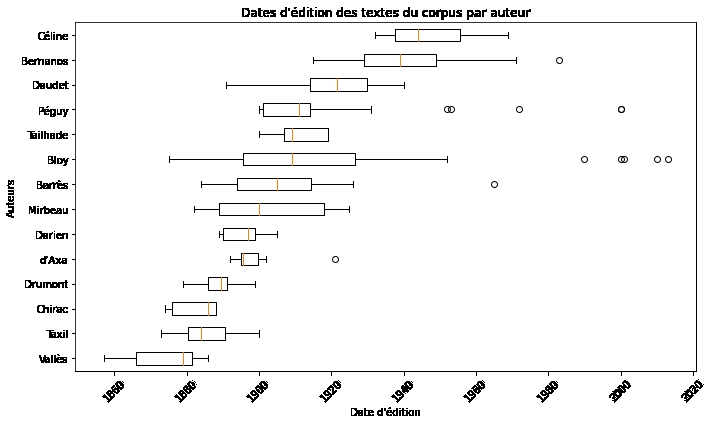
\includegraphics[width=0.85\textwidth]{img/M2_boxplot_corpus_chronologique.jpg}
\caption{\textit{Boite à moustache des dates d'éditions des textes du corpus par auteurs}}
\label{'fig:dates_editions'}
\end{figure}

Ces treize auteurs sont convoqués comme représentant la production pamphlétaire de cette période.  Ce choix est motivé par plusieurs facteurs : la pérennité de leur œuvre, la variété de leur idéologie et propos et l'impact de leur œuvre du vivant de ces écrivains. Ces facteurs restent difficilement mesurables, nous avons néanmoins essayé de représenter plusieurs sons de cloche de ce qu'a pu être la production littéraire pamphlétaire de cette période. 

De nombreuses difficultés n'ont pas pu être éliminés pour cette sélection de textes et la qualification en genre des textes. Une part importante de texte bien que qualifiée par différents acteurs (critiques, journalistes, éditeurs, encyclopédies, etc.) de pamphlet peut relever tout autant d'autres genres proches. Cela est en partie dû à l'ambiguïté et l'absence de définition clair du terme de pamphlet dans la recherche.
Une autre difficulté s'est ajouté pour la constitution de ce corpus quant à l'accessibilité des textes convoqués pour former ce corpus. La majorité des ouvrages sont issus de Wikisource, du projet Gutenberg, de Google Books et de Gallica. À l'exception des textes issus de Wikisource, l'ensemble des textes ont nécessités une étape laborieuse de traitement OCR (Optical Caracter Recognition) car uniquement disponible au format image. Cette conversion du format image au format texte s'est effectué sur les images des textes avec le logiciel Tesseract\footcites{noauthor_tesseract-ocrtesseract_nodate}. Une étape de préparation et de normalisation des images à été effectué avec l'utilitaire ScanTailor. \footcites{noauthor_4lex4scantailor-advanced_nodate}
Sur la figure suivante nous pouvons voir la part d'ouvrage réuni dans le corpus en rapport avec la production réelle identifiée de ces écrivains.
 \begin{figure}[H]
\centering %
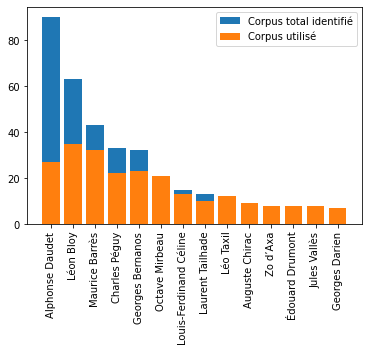
\includegraphics[width=0.85\textwidth]{img/barplot_corpus_auteurs.png}
\caption{\textit{Barplot des textes du corpus par auteurs sur le nombre total de textes identifié de l'auteur.}}
\end{figure}

\subsection{Limites génériques}

Nous avons identifié et réuni en catégorie générique large les différents textes du  corpus. Pour obtenir au maximum des catégories équilibrées, nous avons exclu les quelques pièces de théâtre et les recueils de poésie trop peu nombreux pour former une catégorie comparable aux autres. Cette production textuelle ce découpe en roman, nouvelle, intime, article, essai et pamphlet. Intime étant une catégorie regroupant des biographies, autobiographies et des mémoires. La catégorisation en genre des différents textes est basé sur l'état de l'art bien que certain textes puissent être qualifié par plusieurs étiquettes de genre, notamment certains essais et pamphlets qui sont parfois difficilement discernable les uns des autres sans une connaissance approfondi de leur contenu. Malgré ces difficultés nous avons donc un corpus cohérent de la production littéraire de nos auteurs pamphlétaires. La figure \ref{'fig:repartition_genre'} permet de visualiser le nombre de texte par catégorie générique et par auteur, montrant une distribution homogène, exception faite de la catégorie des nouvelles. 
 \begin{figure}[H]
\centering %
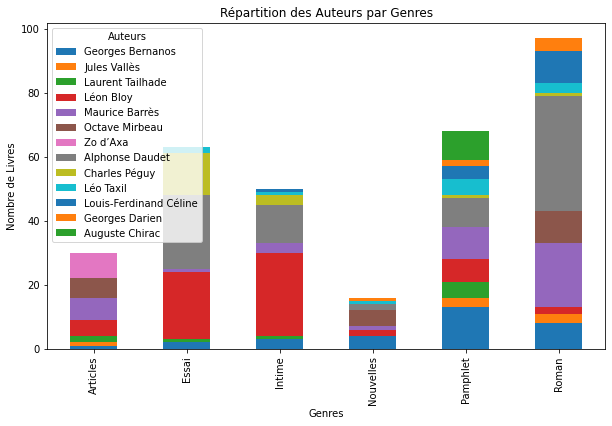
\includegraphics[width=0.65\textwidth]{img/barplot_corpus_genre.png}
\caption{\textit{Barplot de la répartition des auteurs par genre des textes du corpus}}
\label{'fig:repartition_genre'}
\end{figure}

\section{Conclusion}

Le corpus que nous avons constitué nous permettra à lui seul de déployer plusieurs méthodes quantitatives pour étudier le pamphlet. Sa constitution, bien que parfois elle ai nécessité des choix subjectifs et qu'elle soit dépendante de l'accessibilité imparfaite des ouvrages, fut le fruit d'un long travail de sélection des textes et des auteurs les plus représentatifs de la figure du pamphlétaire défini par Marc Angenot. Nous utilisons dans la première partie de cette étude un second corpus complémentaire issu de l'ANR Chapitres des romans du XIX\ieme et XX\ieme siècle, que nous définirons dans cette première partie.

%\footcites{guyot_stylemes_2006}
%\footcites{abbou_genre_2016}
%\footcites{bourdieu_les_1992}
%\footcites{marty_roland_2005}
%\footcites{molinie_style_1996}

%\footcites{molinie_approches_1993}

%\footcites{maingueneau_contexte_1993}

%\footcites{philippe_pourquoi_2021}
%\footcites{philippe_reve_2013}
%\footcites{barthes_degre_1972}
%\footcites{philippe_langue_2009}
%\footcites{jeannelle__2017}
%\footcites{molinie_quest-ce_1994}

%\footcites{angenot_glossaire_nodate}